\begin{enumerate}
    \item Se implementa en MATLAB la  función \texttt{y = interpola(x,P)}, que  interpola una señal realizando los pasos de \textit{upsampling} y filtrado. Donde x es la señal de entrada con una frecuencia de muestreo $Fs$ y P es el factor de \textit{upsampling}, es decir el numero de muestras ceros que se agregan a la señal original  entre sus  muestras (Técnicamente se agregan P-1 ceros).
    
    
    \begin{lstlisting}
    function y = interpola(x,P)
        y = [];
        N = length(x);
        
        %Upsampling
        for i = 1:N
            y = horzcat(y, x(i), zeros(1,P-1));
        end
        
        %Filtrado
        B = fir1(40, 1/P);
        
        %Correccion de Magnitud
        y = P*filter(B,1,y);
    
    end
    \end{lstlisting}
    
    Para visualizar el efecto de la interpolación implementada se realizan pruebas con una señal aleatoria de 10 muestras y utilizando un factor P de 7, obteniendo de esta forma las gráficas presentes en la figura \ref{interpola}. Cabe mencionar que por el efecto de el filtro aplicado se genera un retardo de grupo en la señal resultante, este efecto se muestra en la primera gráfica de la figura, mientras que en la segunda gráfica presenta este mismo resultado pero con el resultado de la interpolación eliminando las muestras correspondientes a este   retardo de grupo.
    
    
    
    
\begin{figure}[H]
    \centering
    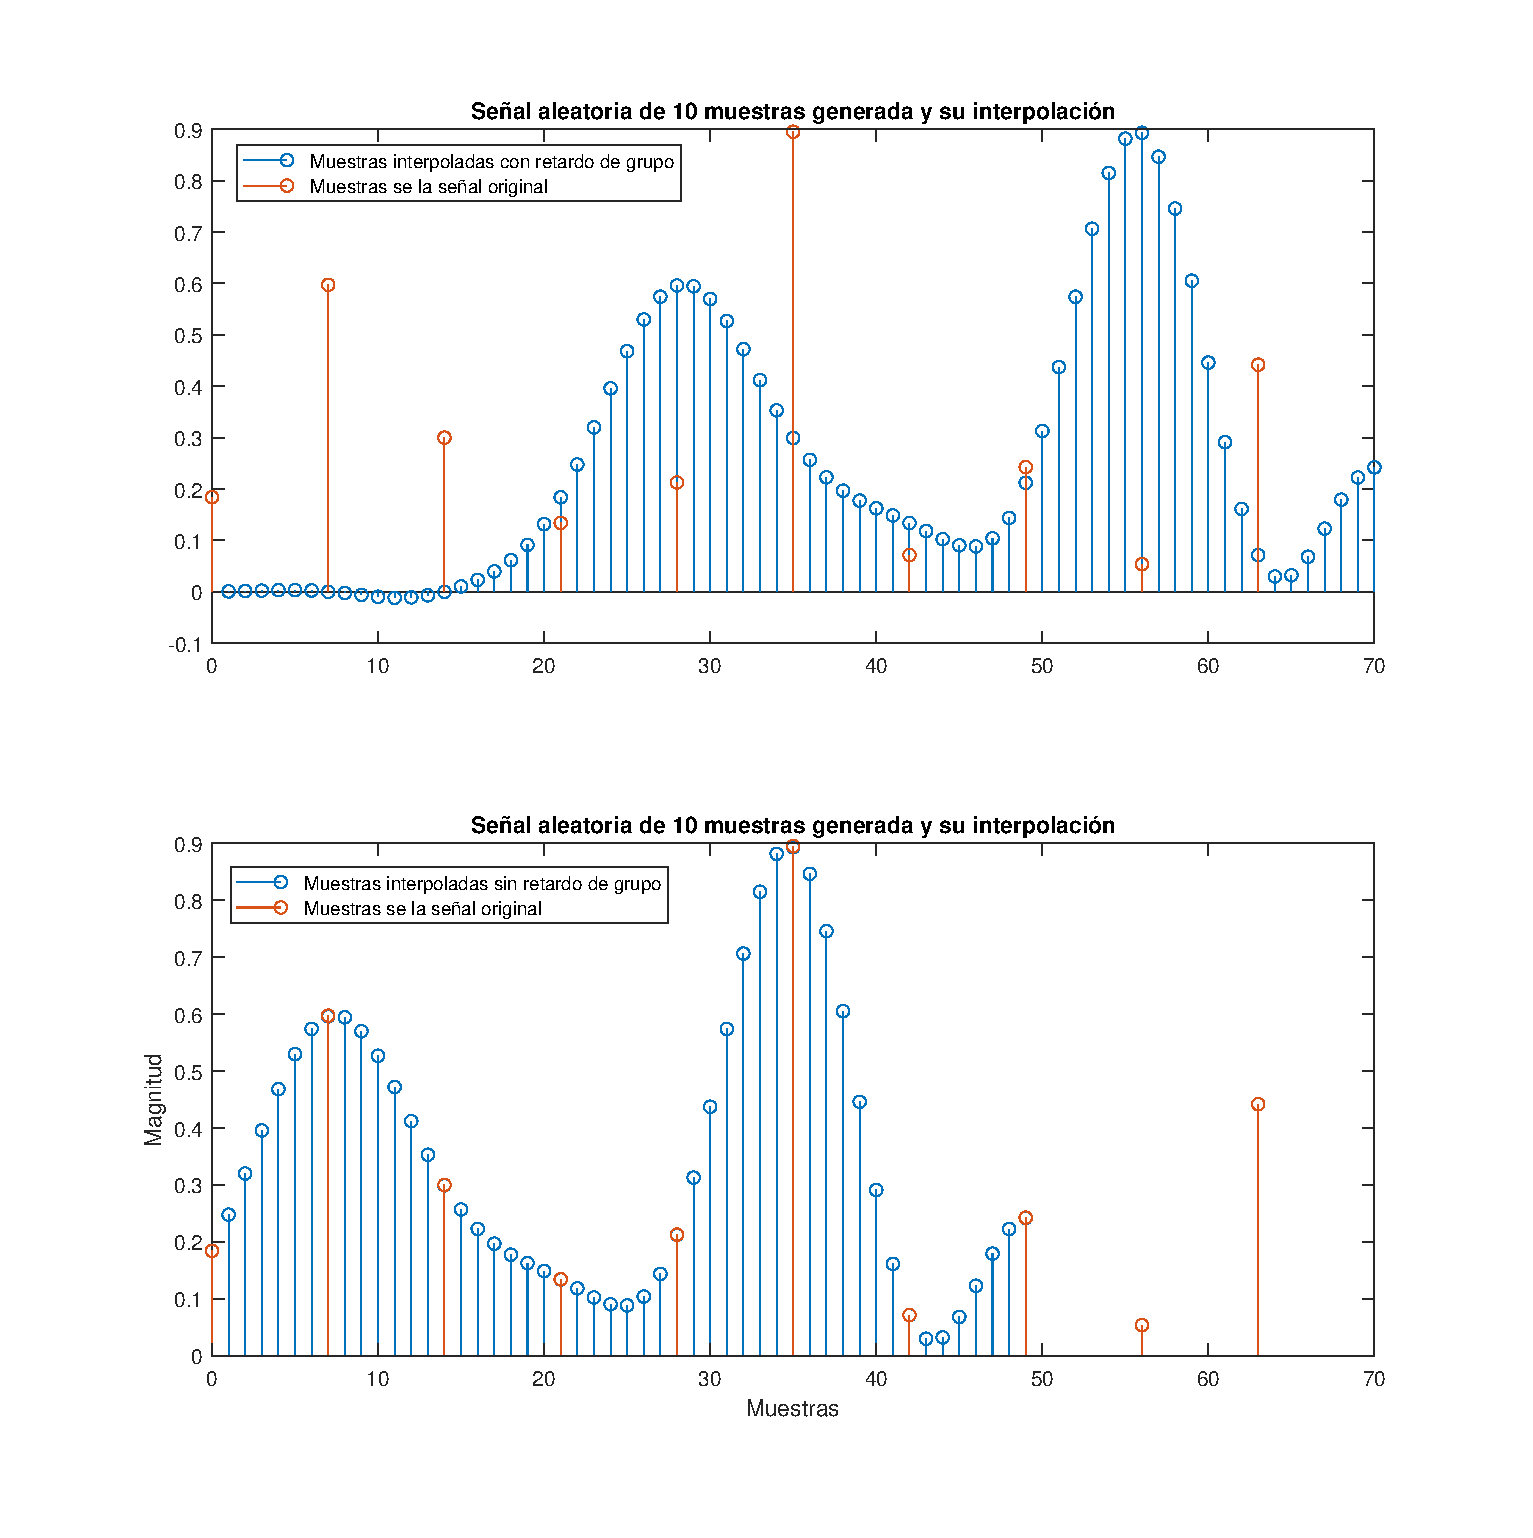
\includegraphics[scale = 0.5]{Figuras/p5_1_interpola.eps}
    \caption{Gráfica de señal aleatoria de 10 muestras junto a su interpolación obtenida.}
    \label{interpola}
\end{figure}
    
    
    Para analizar como va variando el espectro de una señal interpolada  se grafica el espectro obtenido  en  cada paso del proceso de interpolación, esto es, la señal original, la señal luego del \textit{upsampling} y la señal interpolada para el archivo \terxtit{aliasing\_test\_16\_16.mat}. Estas gráficas se muestran en la figura \ref{espectro_inter}, donde se puede ver que el espectro luego del \textit{upsampling} se contrajo  apareciendo la información del espectro a un tercio de la frecuencia a la que aparecía en el espectro de la señal original además de presentar aliases periódicos tal como se  esperaba según la teoría. Finalmente  luego de aplicar el filtro se obtiene el espectro resultante de la  señal interpolada.
    
    
\begin{figure}[H]
    \centering
    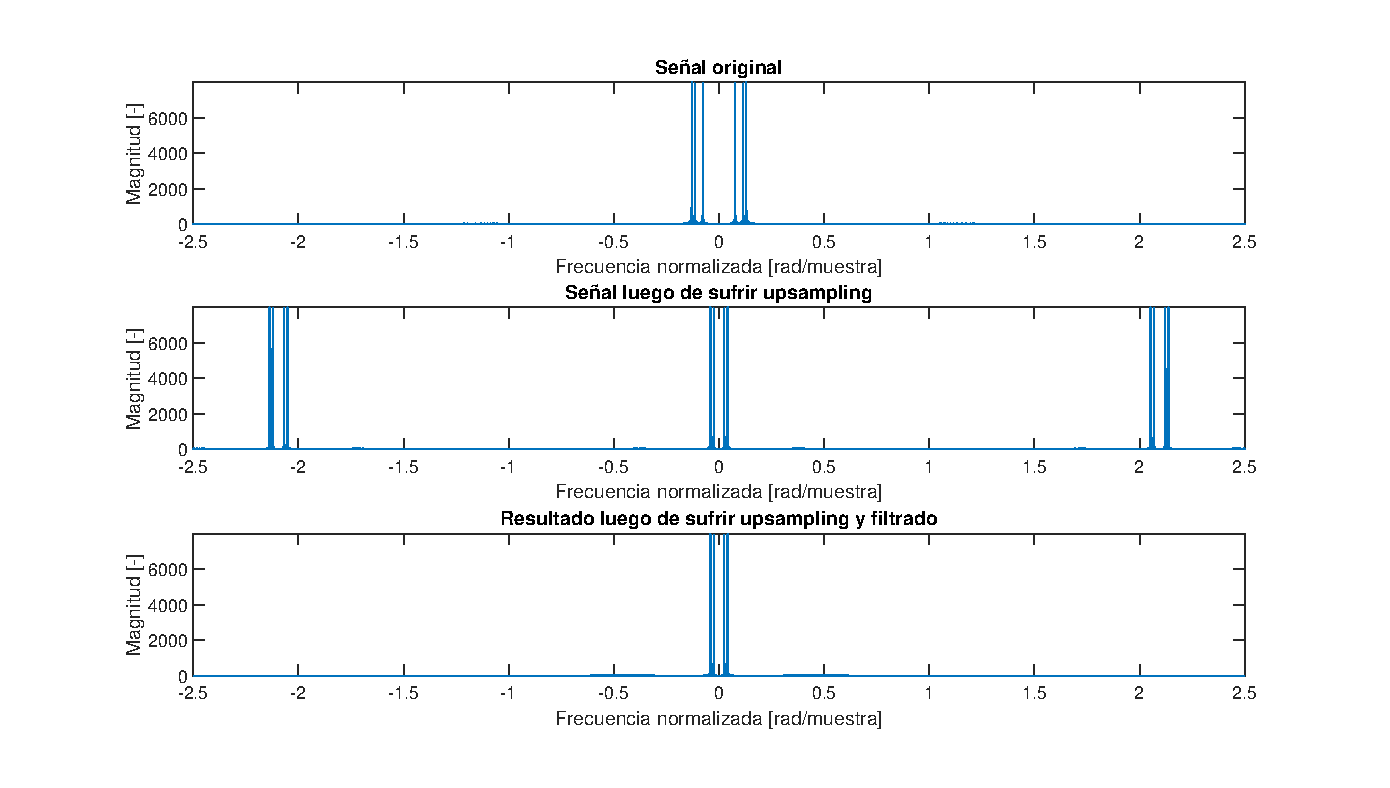
\includegraphics[scale = 0.6]{Figuras/p5_1_espectros.eps}
    \caption{Espectro de los diferentes pasos del proceso de interpolación para el archivo \terxtit{aliasing\_test\_16\_16.mat}}
    \label{espectro_inter}
\end{figure}
    
    
    
Posteriormente se genera una señal Delta de Kronecker en  un vector de muestras donde dicho delta se encuentra en la muestra numero 20,  para poder observar el efecto de la interpolación tanto en muestras anteriores como posteriores al impulso. Esta señal generada se utilizará como entrada al proceso de interpolación que se ha implementado, los resultados obtenidos se muestran en la figura \ref{kroneker}

\begin{figure}[H]
    \centering
    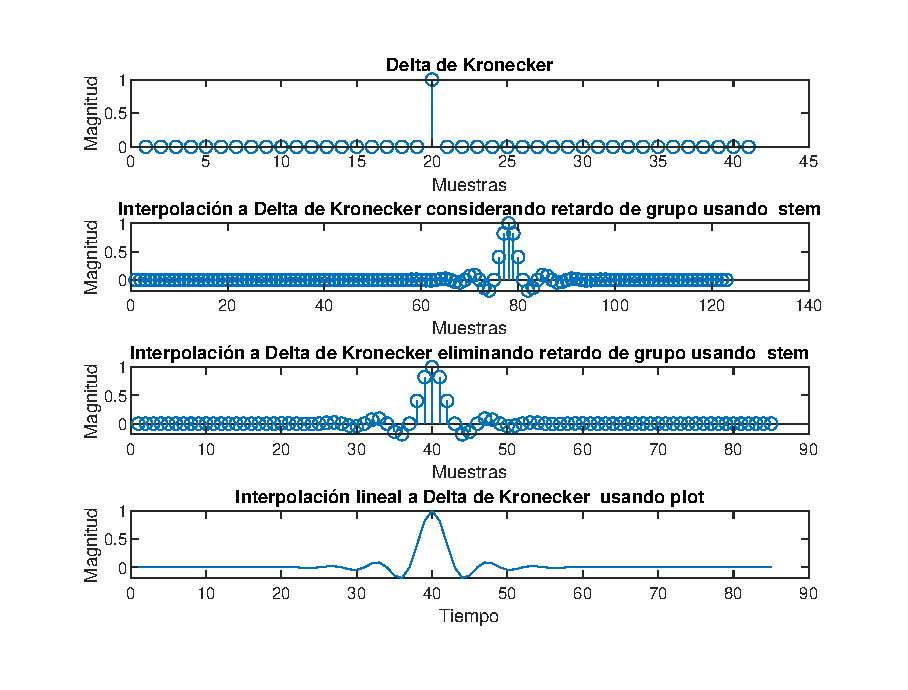
\includegraphics[scale =1]{Figuras/p5_1_kronecker.eps}
    \caption{Interpolación a un Delta de Kronecker.}
    \label{kroneker}
\end{figure}

En la figura anterior se puede ver que la respuesta Y a un impulso de Kronecker se asemeja a una señal \textit{sinc} con el inherente retardo de grupo asociado al filtro (segundo gráfico),ignorando dicho retardo, el resultado  hace sentido, ya que el espectro en frecuencia de un impulso corresponde a una constante que al pasar por un filtro FIR de alto orden (en este caso orden 40), entrega una señal \textit{rect} en frecuencia, al llevar este resultado de vuelta al dominio del temporal se obtiene una teóricamente una señal \textit{sinc}. Se concluye entonces que la respuesta a impulso de  el filtron FIR de orden 40 corresponde a una \terxtit{sinc}.
    
    
    
    
    
\item Se implementa en MATLAB la  función \texttt{y = decima(x,P)}, que  aplica decimación de factor $P$ a la señal de entrada $x$ mediante filtrado y downsampling. La implementación se muestra a continuación:
    
    \begin{lstlisting}
    function Y = decima(X,Q)
        %Filtrado
        B = fir1(40, 1/Q);
        y = filter(B,1,X);        
    
        %Downsampling
        N = round(length(X)/Q);
        Y = zeros(N,1);
        for i = 1:N
            Y(i)= y((i-1)*Q+1);
        end
    
        %Correccion de Magnitud    
        Y = Q*Y;
    end
    \end{lstlisting}

Posteriormente se utiliza la función para procesar la señal \texttt{aliasing\_test} para $Q = 4$ y se grafica la magnitud de la FFT de la señal original y de la señal luego de la decimación. Los gráficos resultantes se muestran en la figura \ref{fig:p5_2}. Se observa el correcto funcionamiento de la función de decimación,  expandiéndose en un factor de $Q$ el ancho del espectro y manteniéndose las amplitudes. 

\begin{figure}[H]
    \centering
    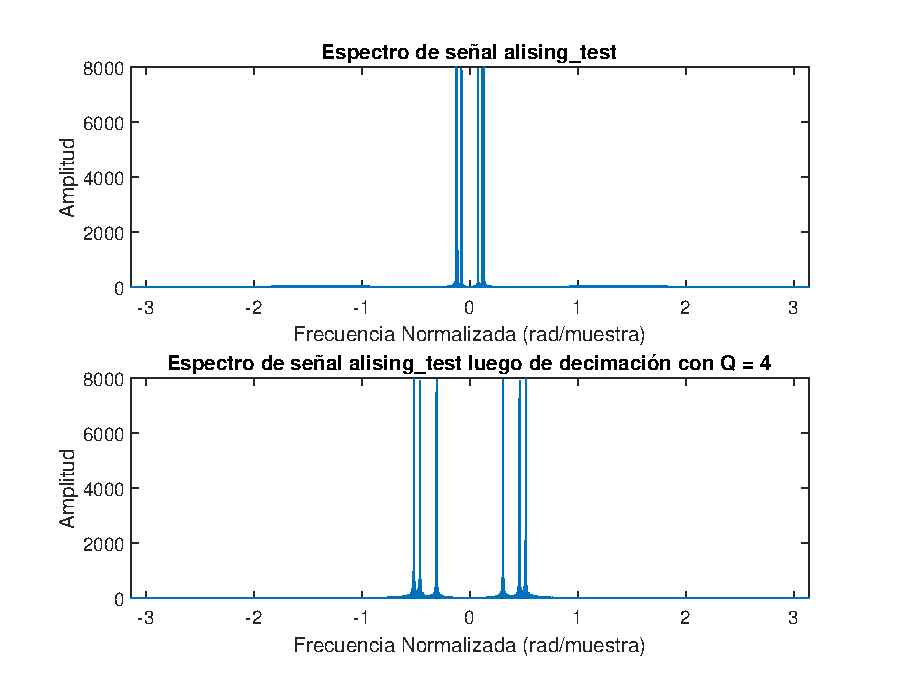
\includegraphics[width = .9\linewidth]{Figuras/p5_2.eps}
    \caption{Espectro de señal \texttt{aliasing\_test} original y luego de aplicar decimación.}
    \label{fig:p5_2}
\end{figure}

\item Se utilizan las funciones de decimación e interpolación para hacer un remuestreo de la señal \texttt{aliasing\_test} desde $16~ksps$ a $12~ksps$.

Para encontrar el factor de decimación se busca llegar a una frecuencia de muestreo que permita llegar a $12~ksps$ usando interpolación. Lo anterior corresponde a encontrar el máximo común divisor entre las frecuencias, por lo tanto el factor de decimación $Q$ está dado por:
$$Q = \dfrac{16k}{\text{M.C.D}(16,12)} = \dfrac{16}{4} = 4 \text{ ksps}$$

Luego el factor $P$ es el necesario para llevar de 4 ksps a 12 ksps, por lo tanto $P = 3$.

Luego se grafica la magnitud de la FFT de la señal original y la señal remuestreada, lo cual se muestra en la figura \ref{fig:p5_3}. Se observa lo esperado en la ''expansión'' del espectro por disminuir la frecuencia de muestreo.

\begin{figure}[H]
    \centering
    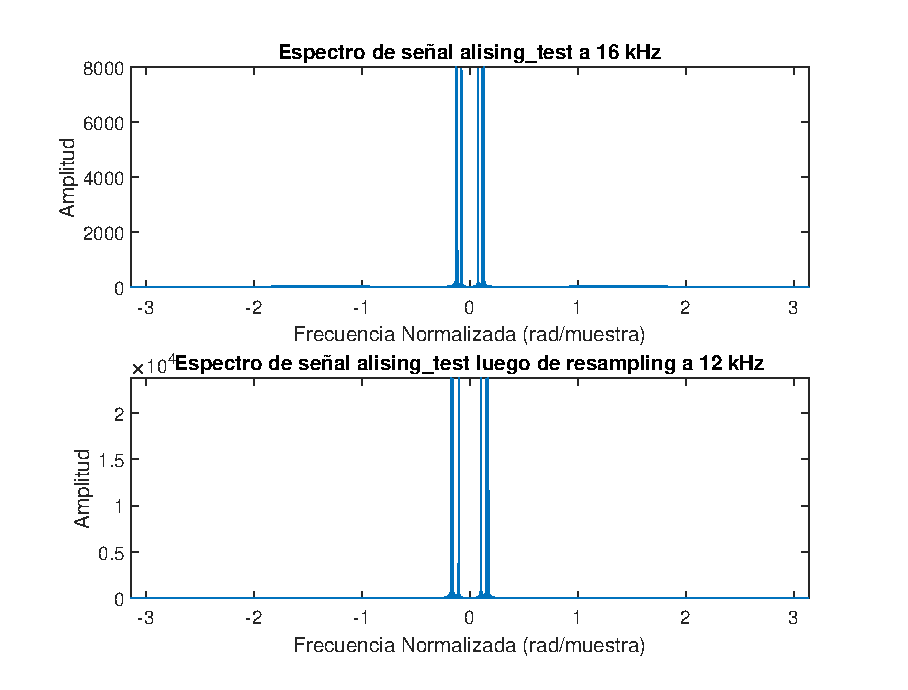
\includegraphics[width = .7 \linewidth]{Figuras/p5_3.eps}    \caption{Espectro de señal \texttt{aliasing\_test} y señal resampleada.}
    \label{fig:p5_3}
\end{figure}

La señal resultante se guarda en el archivo \textit{aliasing\_test\_16\_12.wav} y se adjunta a la entrega.

\end{enumerate}

